%
% problemstellung.tex -- Beispiel-File für die Beschreibung des Problems
%
% (c) 2020 Prof Dr Andreas Müller, Hochschule Rapperswil
%
\section{Iteration der logistischen Gleichung
\label{logistic:section:problemstellung}}
\rhead{Iteration der logistischen Gleichung}

Im Kapitel \ref{buch:section:iteration} haben wir uns
bereits mit dem Iterieren von Funktionen befasst. 
Genau dieses Prinzip der Iteration finden wir auch bei
der logistischen Gleichung wieder. 
Jede Berechnung der Population im Folgejahr ist nämlich
eine Iteration der logistische Gleichung.
Die logistische Gleichung \ref{eq:logistic} könnte man 
auch als Funktion $f(x) = \lambda x(1-x)$ schreiben.
Jede Iteration ist nun eine Verschachtelung von $f(x)$,
somit lässt sich jeder beliebige Wert $x_n$ auch wiefolgt berechnen:
\begin{itemize}
    \item $x_1 = f(x_0)$
    \item $x_2 = f(x_1) = f(f(x_0))$
    \item $x_3 = f(x_2) = f(f(f(x_0)))$
    \item $x_4 = f(x_3) = f(f(f(f(x_0))))$
    \item $x_5 = ...$
\end{itemize}

Wir haben im vorherigen Kapitel bereits beobachtet, 
dass die logistische Gleichung beim Iterieren für 
verschiedene Werte von $\lambda$ gegen verschiedene 
Endwerte konvergiert. 
Der Anfangswert $x_0$ scheint dabei keine Rolle zu spielen
solange er sich im Bereich $0 < x < 1$ befindet, 
er beinflusst lediglich die Form der Kurve, 
bevor sie den Konvergenzwert erreicht. 
Das heisst, wir können $x_0$ auf einen bestimmten Wert, 
zum Beispiel 0.1, setzen. 
Nun können wir $\lambda$ auf einen bestimmten Wert setzen
und die logistische Gleichung endlos iterieren, 
um zu sehen, gegen welchen Wert $x_n$ schliesslich konvergiert.
Mit dem Computer können natürlich nicht unendlich viele Iterationen
durchgeführt werden, aber wenn $n$ gross genug ist, 
kommt man doch sehr nahe an den tatsächlichen Konvergenzwert. 
Genau dieser Prozess ist nun auf Abbildung \ref{fig:pop_logistic} 
ersichtlich. 
Sie zeigt einen Plot, 
auf dem die horizontale Achse die verschiedenen Werte
von $\lambda$ im Bereich für $0 \leq \lambda \leq 4$ annimmt 
und die vertikale Achse anzeigt,
auf welchem Wert $x_n$ konvergiert, wenn $n$ gegen
unendlich läuft. Dabei werden einige Eigenschafen 
von der Iteration der logistischen Gleichung ersichtlich:
\begin{figure}
    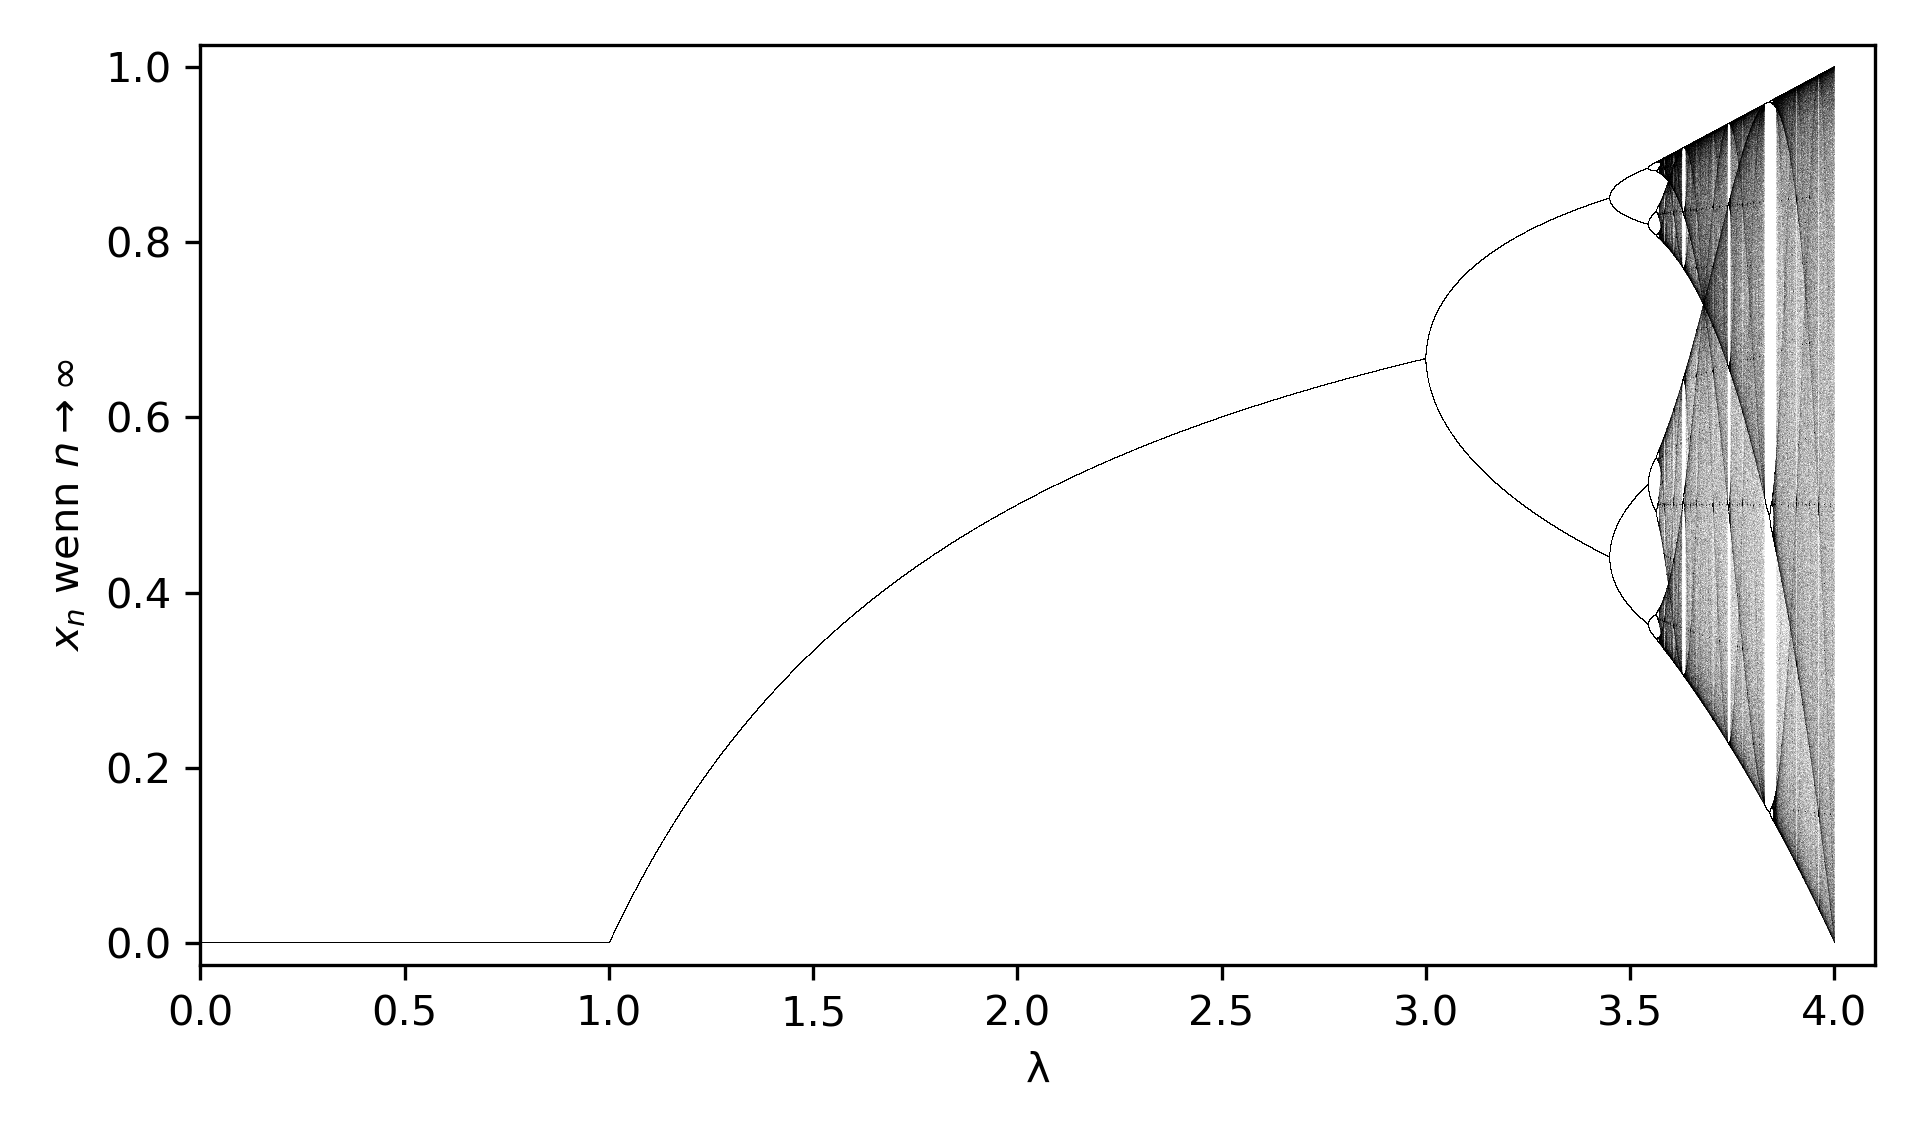
\includegraphics[width=\linewidth]{papers/logistic/figures/map.png}
    \caption{Bifurkationsdiagramm der logistischen Gleichung}
    \label{fig:map_1}
\end{figure}
\begin{itemize}
    \item 
    für $0 \le \lambda \le 1$ konvergiert $x$ gegen 0
    \item 
    für $1 \le \lambda \le 3$ konvergiert $x$ gegen einen fixen Wert
    \item 
    für $\lambda > 3$ scheint $x$ nicht mehr gegen einen fixen Wert zu konvergieren.
    Stattdessen gibt es diese Verzweigungen, 
    die darauf hindeuten, 
    dass $x$ zuerst bis $\lambda \approx 3.4$ zwischen zwei Werten hin und her oszilliert, 
    dann bis $\lambda \approx 3.6$ zwischen vier Werten, dann 8, 16, usw. 
\end{itemize}
\begin{figure}
    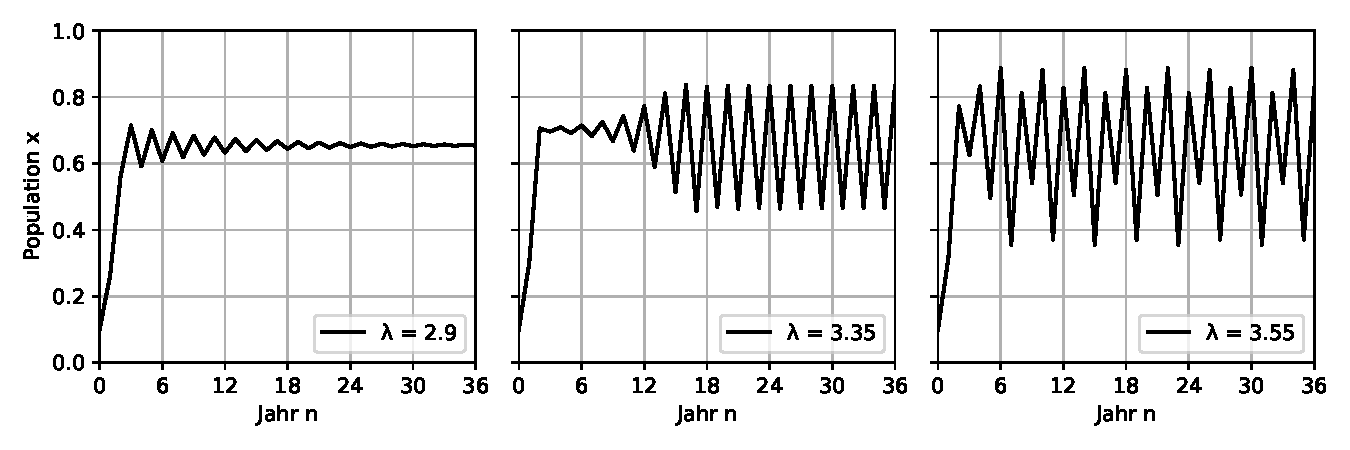
\includegraphics[width=\linewidth]{papers/logistic/figures/pop_logistic_2.pdf}
    \caption{Iteration der logistischen Gleichung}
    \label{fig:pop_logistic_2}
\end{figure}
Das doch eher spezielle Verhalten von $\lambda > 3$ wird 
auch in Abbildung \ref{fig:pop_logistic_2} ersichtlich,
wenn man die Werte der einzelnen Iteration plottet.
Im ersten Plot mit $\lambda = 2.9$ sieht man, dass $x$ zuerst oszilliert,
aber schliesslich auf einen fixen Wert konvergiert.
Auf dem zweiten Plot mit $\lambda = 3.35$ scheint $x$ 
für immer zwischen zwei Werten zu oszillieren und beim
dritten Plot mit $\lambda = 3.55$ sogar zwischen vier Werten. 
Dieses Oszillieren zeigt sich in Abbildung \ref{fig:map_1}
durch die Verzweigungen oder auch ``Bifurkationen''. 
Darum wird es auch ``Bifurkationsdiagramm'' genannt. 


